\documentclass[a4paper]{scrartcl}

\usepackage[sumlimits,intlimits]{amsmath}
%\usepackage{array}
\usepackage{wasysym}
\usepackage{graphicx}
\graphicspath{{images/}}
\usepackage{subfigure}
\usepackage{psfrag}
\usepackage{nicefrac}
\usepackage{comment}
\usepackage[colorlinks,urlcolor=black,linkcolor=black,citecolor=black]{hyperref}

\newcommand{\contactadress}{\href{mailto:ssr@spatialaudio.net}
  {\texttt{ssr@spatialaudio.net}}}

\begin{document}

\sloppy

\title{\Huge Introduction to the\\SoundScape Renderer (SSR)}
\author{Jens Ahrens, Matthias Geier and Sascha Spors\\[2ex]
\contactadress}

\date{\today}

\maketitle

\centerline{
\includegraphics[width=.4\linewidth]{ssr_logo.mps}}

\begin{abstract}
\noindent\textsc{\Large
The SoundScape Renderer (SSR) comes with \mbox{ABSOLUTELY} NO WARRANTY.
The SSR is free software and released under the GNU
General Public License, either version 3 of the License, or (at your option)
any later version. For details, see the enclosed file COPYING or
\url{http://www.gnu.org/licenses/}.
}
\vspace{\baselineskip}

\begin{tabular}{ll}
Copyright \textcopyright\ 2012--2014 & Institut f\"ur Nachrichtentechnik,\\
 & Universit\"at Rostock\\
Copyright \textcopyright\ 2006--2012 & Quality \& Usability Lab,\\
 & Telekom Innovation Laboratories,\\
 & Technische Universit\"at Berlin\\
\end{tabular}
\end{abstract}

\thispagestyle{empty} % no page number on first page

% include your stuff here

\newpage
\tableofcontents

\section{General stuff}

\subsection{Introduction}

The SoundScape Renderer (SSR) is a software framework for real-time spatial
audio reproduction running under GNU/Linux, Mac OS X and possibly some other UNIX
variants.
The current implementation provides Wave Field Synthesis (WFS),
binaural (HRTF-based) reproduction, binaural room (re-)synthesis (BRTF-based
reproduction), head-tracked binaural playback, Ambisonics Amplitude Panning 
(AAP), and Vector Base Amplitude Panning (VBAP).
There are also the slightly exotic Generic Renderer.
For each rendering algorithm there is a separate executable file.
For more details see section~\ref{sec:renderers}.

The SSR is intended as versatile framework for the state-of-the-art
implementation of various spatial audio reproduction techniques. You may use it
for your own academic research, teaching or demonstration activities or whatever
else you like.
However, it would be nice if you would mention the use of the SSR by
e.g.\ referencing~\cite{Geier08:AES} or~\cite{geier2012ssr}.

Note that so far, the SSR only supports two-dimensional reproduction for any
type of renderer. For WFS principally any convex loudspeaker setup
(e.g.\ circles, rectangles) can be used. The loudspeakers should be densely
spaced. For VBAP circular setups are highly recommended. APA does require
circular setups. The binaural renderer can handle only one listener at a time.

\subsection{Quick Start}
\label{sec:quick_start}

After downloading the SSR package, open a shell and use following commands:

\begin{verbatim}
tar xvzf ssr-x.x.x.tar.gz
cd ssr-x.x.x
./configure
make
make install
qjackctl &
ssr my_audio_file.wav
\end{verbatim}

You have to replace \texttt{x.x.x} with the current version number, e.g.\
\texttt{0.4.0}.
With above commands you are performing the following steps:
\begin{itemize}
  \item Unpack the downloaded tarball containing the source-code.
  \item Go to the extracted directory%
    \footnote{Note that most relative paths which are
    mentioned in this document are relative to this folder,
    which is the folder where the SSR tarball was extracted. Therefore,
    e.g.\ the \texttt{src/} directory could be something like
    \texttt{\$HOME/ssr-x.x.x/src/} where ``x'' stands for the 
    version numbers.}.
  \item Configure the SSR.
  \item Install the SSR.
  \item Open the graphical user interface for JACK (\verb+qjackctl+).
    Please click ``Start'' to start the server.
    As alternative you can start JACK with
    \begin{quote}
    \texttt{jackd -d alsa -r 44100}
    \end{quote}
    See section~\ref{sec:running_ssr} and
    \texttt{man jackd} for further options.
  \item Open the SSR with an audio file of your choice. This can be a
    multichannel file.
\end{itemize}
%
This will load the audio file \texttt{my\_audio\_file.wav} and create a virtual
sound source for each channel in the audio file.
By default, the SSR will start with the binaural renderer. Please use headphones
to listen to the generated output!

If you don't need a graphical user interface and you want to dedicate all your
resources to audio processing, try
\begin{quote}
\texttt{ssr --no-gui my\_audio\_file.wav}
\end{quote}
%
For further options, see section~\ref{sec:running_ssr} and \texttt{ssr --help}.

\subsection{Audio Scenes}
\label{sec:audio_scenes}

\subsubsection{Format}

The SSR can open \texttt{.asd} files (refer to section \ref{sec:asdf}) as well
as normal audio files. If an audio file is opened, SSR creates an individual
virtual sound source for each channel which the audio file contains. If a
two-channel audio file is opened, the resulting virtual sound sources are
positioned like a virtual stereo loudspeaker setup with respect to the location
of the reference point. For audio files with more (or less) channels, SSR randomly
arranges the resulting virtual sound sources.
All types that
ecasound and libsndfile can open can be used. In particular this includes \texttt{.wav}, \texttt{.aiff}, \texttt{.flac} and \texttt{.ogg} files.

In the case of a scene being loaded from an \texttt{.asd} file, all audio files
which are associated to virtual sound sources are replayed in parallel and
replaying starts at the beginning of the scene. So far, a dynamic handling of
audio files has not been implemented.

\subsubsection{Coordinate System}

\begin{figure}
\psfrag{alpha}{$\alpha$} \psfrag{r}{$r$} \psfrag{x}{$x$}
\psfrag{y}{$y$} \psfrag{bx}{${\bf x}$}
\psfrag{alphaprime}{$\alpha'$}\psfrag{yprime}{$y'$} \psfrag{xprime}{$x'$}
\begin{center}
\subfigure[\label{fig:global_coordinate_system}{Global coordinate system.}]
{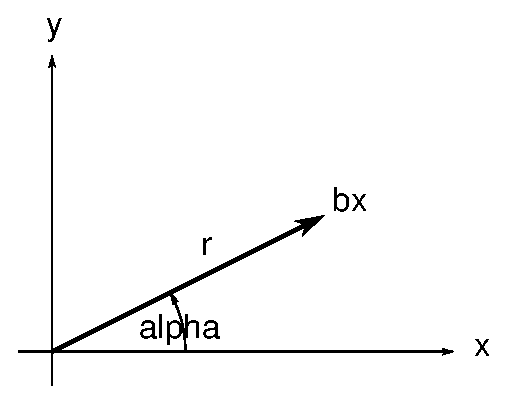
\includegraphics[width=.45\linewidth]{images/coordinate_system.eps}} \hfill
\subfigure[\label{fig:local_coordinate_system}{Local coordinate system relative
to the reference. The latter is indicated by the rhomb.}]
{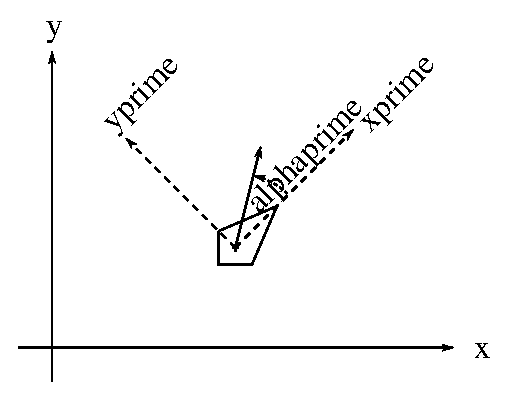
\includegraphics[width=.45\linewidth]{images/local_coordinate_system.eps}}
\caption{\label{fig:coordinate_system}{The coordinate system used in the SSR.
In ASDF $\alpha$ and $\alpha'$ are referred to as azimuth (refer to section
\ref{sec:asdf}).}}
\end{center}
\end{figure}

Fig.~\ref{fig:global_coordinate_system} depicts the global coordinate system
used in the SSR. Virtual sound sources as well as the reference are positioned
and orientated with respect to this coordinate system. For loudspeakers,
positioning is a bit more tricky since it is done with respect to a local
coordinate system determined by the reference. Refer to 
Fig.~\ref{fig:local_coordinate_system}. The loudspeakers are positioned with 
respect to the primed coordinates ($x'$, $y'$, etc.).

The motivation to do it like this is to have a means to virtually move the
entire loudspeaker setup inside a scene by simply moving the reference. This
enables arbitrary movement of the listener in a scene independent of the
physical setup of the reproduction system.

Please do not confuse the origin of the coordinate system with the reference. 
The coordinate system is static and specifies absolute positions.

The reference is movable and is always taken with respect to the current 
reproduction setup. The loudspeaker-based methods do not
consider the orientation of the reference point but its location influences the
way loudspeakers are driven. E.g., the reference location corresponds to the
\emph{sweet spot} in VBAP. It is therefore advisable to put the reference point
to your preferred listening position. In the binaural methods
the reference point represents the listener and indicates the position and 
orientation of the latter. It is therefore essential to set it properly in this
case.

Note that the reference position and orientation can of course be updated in
real-time. For the loudspeaker-based methods this is only useful to a limited
extent unless you want to move inside the scene. However, for the binaural 
methods it is essential that both the reference position and orientation 
(i.e.\ the listener's position and orientation) are tracked and updated in 
real-time. Refer also to Sec.~\ref{sec:head_tracking}.

\subsection{Audio Scene Description Format (ASDF)}
\label{sec:asdf}

Besides pure audio files, SSR can also read the current development version of
the \emph{Audio Scene Description Format
(ASDF)}~\cite{Geier08:DAGA}. Note however that so
far, we have only implemented descriptions of static features. That
means in the current state it is not possible to describe
e.g.~movements of a virtual sound source. As
you can see in the example audio scene below, an audio file can be
assigned to each virtual sound source. The replay of all involved
audio files is synchronized to the replay of the entire scene. That
means all audio files start at the beginning of the sound scene. If
you fast forward or rewind the scene, all audio files fast forward
or rewind. {\bf Note that it is sigificantly more efficient to read data from
an interleaved multichannel file compared to reading all channels from
individual files}.

\subsubsection{Syntax}

The format syntax is quite self-explanatory. See the examples below.
Note that the paths to the audio files can be either absolute (not
recommended) or relative to the directory where the scene file is
stored. The exact format description of the ASDF can be found in the
XML Schema file \texttt{asdf.xsd}.

\noindent Find below a sample scene description:

\begin{verbatim}
<?xml version="1.0"?>
<asdf version="0.1">
  <header>
    <name>Simple Example Scene</name>
  </header>
  <scene_setup>
    <source name="Vocals" model="point">
      <file>audio/demo.wav</file>
      <position x="-2" y="2"/>
    </source>
    <source name="Ambience" model="plane">
      <file channel="2">audio/demo.wav</file>
      <position x="2" y="2"/>
    </source>
  </scene_setup>
</asdf>
\end{verbatim}

\noindent The input channels of a soundcard can be used by specifying the
channel number instead of an audio file, e.g. \verb|<port>3</port>| instead of
\verb|<file>my_audio.wav</file>|.

\subsubsection{Examples}

We provide an audio scene example in ASDF with this release. You find it in
\texttt{data/scenes/live\_input.asd}. If you load this file into the SSR it
will create 4 sound sources which will be connected to the first four channels
of your sound card. If your sound card happens to have less than four outputs, less sources will be created accordingly.
More examples for audio scenes can be downloaded from the SSR
website~\cite{ssr}.

\subsection{IP Interface}

\label{sec:ip_interface}

One of the key features of the SSR is an interface which lets you
remotely control the SSR via a TCP socket using XML messages. This
interface enables you to straightforwardly connect any type of
interaction tool from any type of operating system.
The format of the messages sent over the network is still under development and
may very likely change in future versions.
Please find some
brief information in section~\ref{sec:network}.

%An example how the SSR can be controlled via its network interface is the
%Python client located in the directory \verb|python_client/| and the provided
%Pure Data patches.

\subsection{Bug Reports, Feature Requests and Comments}

%For a list of known problems have a look at the SSR development website%
%\footnote{\url{https://dev.qu.tu-berlin.de/projects/ssr/wiki/Known_Issues}}.
Please report any bugs, feature requests and comments to
\contactadress. We will keep track of them and will try to fix them
in a reasonable time. The more bugs you report the more we can fix.
Of course, you are welcome to provide bug fixes.~\smiley

\subsection{Contributors}

\IfFileExists{authors.tex}{\input{authors}}{%
For a list of contributors, please see the file \texttt{AUTHORS}.}

\subsection{Your Own Contributions}

The SSR is thought to provide a state of the art implementation of
various spatial audio reproduction techniques. We therefore would
like to encourage you to contribute to this project since we can
not assure to be at the state of the art at all times ourselves.
Everybody is welcome to contribute to the development of the SSR.
However, if you are planning to do so, we kindly ask you to contact
us beforehand (e.g.~via \contactadress). The SSR is in a rather
temporary state and we might apply some changes to its architecture.
We would like to ensure that your own implementations stay compatible
with future versions.

\begin{comment}
\subsection{Version history}

\begin{itemize}
\item Initial release: 0.1
\end{itemize}
\end{comment}

\section{Compiling and running the SSR}

\subsection{Mac OSX App-Bundle}

The following sections are relevant if you want to build the SSR from its source
code. This is the default procedure for GNU/Linux systems. If you want to use
the SSR on a Mac, you can also use the pre-compiled app bundle.
For further information visit the SSR website~\cite{ssr}.

\subsection{Getting the Source}

If you didn't receive this manual with the source code of the SSR, you can
download it from the SSR website~\cite{ssr}. After downloading, you can unpack the tarball with
the command \verb+tar xvzf ssr-x.x.x.tar.gz+ in a shell. This will extract the
source code to a directory of the form \verb+ssr-x.x.x+ where ``x'' stands for
the version numbers.  \verb+cd+ to this directory and proceed with section
\ref{sec:configuring} to configure the SSR.

\subsection{Configuring}
\label{sec:configuring}

To build the SSR from source you have to configure first. Open a shell and
\verb+cd+ to the directory containing the source code
%\footnote{Note that the
%top directory of the SSR-package distributed e.g. in a tar-ball is intended.}
of the package and type:

\begin{verbatim}
./configure
\end{verbatim}

This script will check your system for dependencies and prepare the
\verb+Makefile+ required for compilation. Section \ref{sec:dependencies} lists
the dependencies that must be installed on your system. The \texttt{configure} script
will signal if dependencies are missing. At successful termination of the 
\texttt{configure} script a summary will show up.

Section \ref{sec:hints_conf} is intended to help you troubleshooting.

\subsubsection{Dependencies}
\label{sec:dependencies}
At least the following software (libraries and headers) including their
development packages (\emph{dev} or \emph{devel}),
where available, are required for a full installation of the SSR:

\begin{itemize}
\item[-] JACK Audio Connection Kit \cite{jack}
\item[-] FFTW3 compiled for single precision (\texttt{fftw3f}) version 3.0 or higher
  \cite{fftw3}
\item[-] libsndfile \cite{sndfile}
\item[-] Ecasound \cite{ecasound}
\item[-] Trolltech's Qt 4.2.2 or higher with OpenGL (QtCore, QtGui and QtOpenGL)
  \cite{qt4}
%\item[-] GLUT \cite{glut} or freeglut \cite{freeglut}
\item[-] libxml2 \cite{libxml2}
\item[-] Boost.Asio \cite{boost}, included since Boost version 1.35.
\end{itemize}

We provide a simple integration of several head tracking systems.
Please read section
%\ref{sec:configuring} for an actual configuration or read section
\ref{sec:head_tracking} for further informations about head tracking.

\subsubsection{Hints on Configuration}
\label{sec:hints_conf}

If you encounter problems configuring the SSR these hints could help:
\begin{itemize}
\item Ensure that you really installed all libraries (\verb+lib+) with devel-package (\verb+devel+ or \verb+dev+, where available) mentioned in section \ref{sec:dependencies}.
\item It may be necessary to run \verb+ldconfig+ after installing new libraries.
\item Ensure that \verb+/etc/ld.so.conf+ or \verb+LD_LIBRARY_PATH+ are set
  properly, and run \verb+ldconfig+ after changes.
\item If a header is not installed in the standard paths of your system you
  can pass its location to the configure script using
  \verb+./configure CPPFLAGS=-Iyourpath+.
\end{itemize}

Note that with \verb+./configure --help+ all configure-options are displayed,
e.g. in section ``Optional Features'' you will find how to
%enable optimization by compiler, how to
disable compilation of the head trackers
%or how to start the SSR with a different renderer.
and many other things.
Setting the influential environment variables with
\verb+./configure VARNAME=value+ can be useful for debugging dependencies.

\subsection{Compiling and Installing}
\label{sec:comp_inst}

If the configure script terminates with success, it creates a file named 
\texttt{Makefile}. You can build the SSR by typing

\begin{quote}
\texttt{make}\\
\texttt{make install}
\end{quote}
%
This will compile the SSR and install it to your system.
%Section \ref{sec:configuring} contains more information about configuring.

\subsection{Uninstalling}

If the SSR didn't meet your expectations, we are very sorry, and of course you
can easily remove it from your system with
\begin{quote}
\texttt{make uninstall}
\end{quote}

\subsection{Running the SSR}
\label{sec:running_ssr}

Before you start the SSR, start JACK \cite{jack}, e.g.~by typing\\
\verb+jackd -d alsa -r 44100+ in a shell or using the graphical user
interface ``qjackctl'' \cite{qjackctl}.
Now, the easiest way to get a signal out of the SSR is
by passing a sound-file directly:

\begin{quote}
\begin{verbatim}
ssr YOUR_AUDIO_FILE
\end{verbatim}
\end{quote}

By default, the SSR starts with the binaural renderer; please use
headphones for listening with this renderer.
Type \verb+ssr --help+ to get an overview of the command
line options and various renderers:

{\footnotesize
\begin{verbatim}
USAGE: ssr [OPTIONS] <scene-file>

The SoundScape Renderer (SSR) is a tool for real-time spatial audio reproduction
providing a variety of rendering algorithms.

OPTIONS:

Choose a rendering algorithm:
    --binaural         Binaural (using HRIRs)
    --brs              Binaural Room Synthesis (using BRIRs)
    --wfs              Wave Field Synthesis
    --aap              Ambisonics Amplitude Panning
    --vbap             Stereophonic (Vector Base Amplitude Panning)
    --generic          Generic Renderer
    --nfc-hoa          Near-field-corrected Higher Order Ambisonics (experimental!)

Renderer-specific options:
    --hrirs=FILE       Load the HRIRs for binaural renderer from FILE
    --hrir-size=VALUE  Maximum IR length (binaural and BRS renderer)
    --prefilter=FILE   Load WFS prefilter from FILE
-o, --ambisonics-order=VALUE Ambisonics order to use (default: maximum)
    --in-phase-rendering     Use in-phase rendering for Ambisonics

JACK options:
-n, --name=NAME        Set JACK client name to NAME
    --input-prefix=PREFIX    Input  port prefix (default: "system:capture_")
    --output-prefix=PREFIX   Output port prefix (default: "system:playback_")
-f, --freewheel        Use JACK in freewheeling mode

General options:
-c, --config=FILE      Read configuration from FILE
-s, --setup=FILE       Load reproduction setup from FILE
    --threads=N        Number of audio threads (default N=1)
-r, --record=FILE      Record the audio output of the renderer to FILE
    --loop             Loop all audio files
    --master-volume-correction=VALUE
                       Correction of the master volume in dB (default: 0 dB)
-i, --ip-server[=PORT] Start IP server (default on)
                       A port can be specified: --ip-server=5555
-I, --no-ip-server     Don't start IP server
-g, --gui              Start GUI (default)
-G, --no-gui           Don't start GUI
-t, --tracker=TYPE     Start tracker, possible value(s): polhemus vrpn razor
    --tracker-port=PORT
                       A serial port can be specified, e.g. /dev/ttyS1
-T, --no-tracker       Don't start tracker

-h, --help             Show this very help information. You just typed that!
-v, --verbose          Increase verbosity level (up to -vvv)
-V, --version          Show version information and exit
\end{verbatim}
}

Choose the appropriate arguments and make sure that your amplifiers
are not turned too loud\dots

To stop the SSR use either the options provided by the GUI (section
\ref{sec:gui}) or type \texttt{Crtl+c} in the shell in which you started the
SSR.

\paragraph{Keyboard actions in non-GUI mode}

If you start SSR without GUI (option \verb+--no-gui+), it starts automatically
replaying the scene you have loaded. You can have some interaction via the
shell. Currently implemented actions are (all followed by \texttt{Return}):

\begin{itemize}
\item[] \texttt{c}: calibrate tracker (if available)
\item[] \texttt{p}: start playback
\item[] \texttt{q}: quit application
\item[] \texttt{r}: ``rewind''; go back to the beginning of the current scene
\item[] \texttt{s}: stop (pause) playback
\end{itemize}
%
Note that in non-GUI mode, audio processing is always taking place. Live inputs
are processed even if you pause playback.

\paragraph{Recording the SSR output}

You can record the audio output of the SSR using the \texttt{--record=FILE} command
line option. All output signals (i.e.\ the loudspeaker signals) will be recorded
to a multichannel wav-file named \texttt{FILE}. The order of channels
corresponds to the order of loudspeakers specifed in the reproduction setup
(see sections \ref{sec:reproduction_setups} and \ref{sec:asdf}). The recording
can then be used to analyze the SSR output or to replay it without the SSR
using a software player like \texttt{ecaplay}~\cite{ecasound}.

\subsection{Configuration File}
\label{sec:ssr_configuration_file}

The general configuration of the SSR (if GUI
is enabled, which tracker to use etc.) can be specified in a configuration file
(e.g. \texttt{ssr.conf}). By specifying
your settings in such a file, you avoid having to give explicit command
line options every time you start the SSR. We have added the example
\texttt{data/ssr.conf.example} which mentions all possible parameters.
Take a look inside, it is rather self-explanatory.
There are three possibilities to specify a configuration file:
\begin{itemize}
\item put it in \texttt{/etc/ssr.conf}
\item put it in your home directory in \texttt{\$HOME/.ssr/ssr.conf}
\item specify it on the command line with \texttt{ssr -c my\_config.file}
\end{itemize}

We explicitly mention one parameter here which might be of immediate interest
for you: \texttt{MASTER\_VOLUME\_CORRECTION}. This a correction in dB~(!) which is
applied -- as you might guess -- to the master volume. The motivation is to have
means to adopt the general perceived loudness of the reproduction of a given
system. Factors like the distance of the loudspeakers to the listener or the
typical distance of virtual sound sources influence the resulting loudness
which can be adjusted to the desired level by means of the
\texttt{MASTER\_VOLUME\_CORRECTION}. Of course, there's also a command line
alternative (\texttt{--master-volume-correction}).

\subsection{Head Tracking}
% TODO: update this section.
\label{sec:head_tracking}

We provide integration of the \emph{InterSense InertiaCube3} tracking sensor
\cite{intersense} and the  \emph{Polhemus Fastrak}~\cite{fastrack}. They are used to
update the orientation of the reference (in binaural reproduction this is the
listener) in real-time. Please read sections \ref{sec:prep_isense} and
\ref{sec:prep_pol} if you want to compile the SSR with the support for these
trackers.

Note that on startup, the SSR tries to find the tracker. If it fails, it
continues without it. If you use a tracker, make sure that you have the
appropriate rights to read from the respective port.

You can calibrate the tracker while the SSR is running by pressing
\texttt{Return}.
The instantaneous
orientation will then be interpreted as straight forward ($\alpha = 90^\circ$).

\subsubsection{Preparing InterSense InertiaCube3}
\label{sec:prep_isense}

If you want to compile the SSR with support for the \emph{InterSense
InertiaCube3}
tracking sensor~\cite{intersense}, please download the \emph{InterSense Software
Development Kit} (SDK) from the InterSense website~\cite{intersense}.
Unpack the archive and place the files

\begin{itemize}
\item \verb+isense.h+ and \verb+types.h+ to \verb+/usr/local/include+, and
\item \verb+libisense.so+
  %(either from folder \texttt{x86} or \texttt{x86\_64})
  (the version appropriate for your processor type)
  to \verb+usr/local/lib+.
\end{itemize}
%
The SSR \texttt{configuration} script will automatically detect the presence of
the files described above and if they are found, enable the compilation for the 
support of this tracker. To disable this tracker, use 
\verb+./configure --disable-intersense+ and recompile.

If you encounter an error-message similar to \texttt{libisense.so: cannot open 
shared object file: No such file or directory}, but the file is placed 
correctly, run \verb|ldconfig|. 

\subsubsection{Preparing Polhemus Fastrack}
\label{sec:prep_pol}
For incorporation of the \emph{Polhemus Fastrack}~\cite{fastrack} with serial
connection, no additional libraries are required.
%The files
%\verb+termios.h,unistd.h, fcntl.h and poll.h+ should be already installed on
%your system. If they are found, the configure-script will enable the
%compilation for the support of this tracker.
If you want to disable this
tracker, use \verb+ ./configure --disable-polhemus+ and recompile.

\subsection{Using the SSR with DAWs}

As stated before, the SSR is currently not able to dynamically replay audio
files (refer to section~\ref{sec:asdf}). If your audio scenes are complex, you
might want to consider using the SSR together with a digital audio work station
(DAW). To do so, you simply have to create as many sources in the SSR as you
have audio tracks in your respective DAW project and assign live inputs to the
sources. Amongst the ASDF examples we provide at~\cite{ssr} you find an example
scene description which does exactly this.

DAWs like Ardour~\cite{ardour} support JACK and their use is therefore straightforward. DAWs which do not run on Linux or do not support JACK can be connected
via the input of the sound card.

In the future we will provide a VST plug-in which will allow you to dynamically
operate all virtual source's properties (like e.g.~a source's position or level
etc.). You will then be able to have the full SSR functionality controlled from your
DAW.

\section{The Renderers}
\label{sec:renderers}

\subsection{General}

\subsubsection{Reproduction Setups}
\label{sec:reproduction_setups}

The geometry of the actual reproduction setup is specified in
\texttt{.asd} files, just like sound scenes. By default, it is loaded from the
file \texttt{/usr/local/share/ssr/default\_setup.asd}.
Use the \texttt{--setup} command line option to load another reproduction setup file.
Note that the
loudspeaker setups have to be convex. This is not checked by the SSR.
The loudspeakers appear at the outputs of your sound card in the same
order as they are specified in the \texttt{.asd} file, starting with channel 1.

\noindent A sample reproduction setup description:

\begin{verbatim}
<?xml version="1.0"?>
<asdf version="0.1">
  <header>
    <name>Circular Loudspeaker Array</name>
  </header>
  <reproduction_setup>
    <circular_array number="56">
      <first>
        <position x="1.5" y="0"/>
        <orientation azimuth="-180"/>
      </first>
    </circular_array>
  </reproduction_setup>
</asdf>
\end{verbatim}

\noindent We provide the following setups in the directory
\verb+data/reproduction_setups/+:
\begin{itemize}
\item[-] \texttt{2.0.asd}: standard stereo setup at 1.5 mtrs distance
\item[-] \texttt{2.1.asd}: standard stereo setup at 1.5 mtrs distance plus subwoofer
\item[-] \texttt{5.1.asd}: standard 5.1 setup on circle with a diameter of 3 mtrs
\item[-] \texttt{rounded\_rectangle.asd}: Demonstrates how to combine circular
	arcs and linear array segments.
\item[-] \texttt{circle.asd}: This is a circular array of 3 mtrs diameter
	composed of 56 loudspeakers.
\item[-] \texttt{loudspeaker\_setup\_with\_nearly\_all\_features.asd}: This
	setup describes all supported options, open it with your favorite text
	editor and have a look inside.
\end{itemize}

\noindent Note that outputs specified as subwoofers receive a signal having
full bandwidth.
There is some limited freedom in assigning channels to loudspeakers:
If you insert the element \texttt{<skip number="5"/>},
the specified number of output channels are skipped and the following
loudspeakers get higher channel numbers accordingly.

Of course, the binaural and BRS renderers do not load a loudspeaker setup. By
default, they assume the listener to reside in the coordinate origin looking
straight forward.

\subsubsection{A Note on the Timing of the Audio Signals}

The WFS renderer is the only renderer in which the timing of the audio signals is 
somewhat peculiar. None of the other renderers imposes any algorithmic delay on 
individual source signals. Of course, if you use a renderer which is convolution 
based such as the BRS renderer, the employed HRIRs do alter the timing of the 
signals due to their inherent properties. 

This is different with the WFS renderer. Here, also the propagation duration of 
sound from the position of the virtual source to the loudspeaker array is 
considered. That means that the farther a virtual source is located, the longer
is the delay imposed on its input signal. This also holds true for plane waves: 
Theoretically, plane waves do originate from infinity. Though, the SSR does consider
the origin point of the plane wave which is specified in ASDF. This origin point 
also specifies the location of the symbol which represents the respective plane
wave in the GUI. 

We are aware that this procedure can cause confusion and reduces the ability of
a given scene of translating well between different types of renderers. In the 
upcoming version~0.4 of the SSR we will implement an option that will allow you 
specifying for each individual source whether the propagation duration of sound 
shall be considered by a renderer or not. 

\subsubsection{Distance Attenuation}

Note that in all renderers -- except the BRS renderer -- distance attenuation
is handled as $\nicefrac{1}{r}$ with respect to the distance $r$ of the
respective virtual source to the reference position. Sources closer than 0.5
mtrs to the reference position do not experience any increase of amplitude.
Virtual plane waves do not experience any algorithmic distance attenuation in
any renderer.
In future versions of the SSR more freedom in specifying the distance attenuation 
will be provided.

The amplitude reference distance, i.e.~the distance from the reference at which
plane waves are as loud as the other source types (like point sources), can be
set in the SSR configuration file (Section~\ref{sec:ssr_configuration_file}).
The desired amplitude reference distance for a given sound scene can be
specified in the scene description (Section~\ref{sec:asdf}). The default value
is 3~m.

\subsubsection{Doppler Effect}

In the current version of the SSR the Doppler Effect in moving sources is not
supported by any of the renderers.

\subsubsection{Signal Processing}

All rendering algorithms are implemented on a frame-wise basis with an internal
precision of 32 bit floating point. The signal processing is illustrated in
Fig.~\ref{fig:signal_processing}.

The input signal is divided into individual frames of size \emph{nframes}, whereby
\emph{nframes} is the frame size with which JACK is running. Then e.g.\ frame number
$n+1$ is processed both with previous rendering parameters $n$ as well as with
current parameters $n+1$. It is then crossfaded between both processed frames
with cosine-shaped slopes. In other words the effective frame size of the
signal processing is $2\cdot\text{\emph{nframes}}$ with 50\% overlap. Due to the fade-in of
the frame processed with the current parameters $n+1$, the algorithmic latency
is slightly higher than for processing done with frames purely of size
\emph{nframes} and no crossfade.

\begin{figure}
\footnotesize \psfrag{input}{\bf input signal} \psfrag{output}{\bf
output signal} \psfrag{dots}{\bf \dots} \psfrag{+}{\bf +}
\psfrag{n}{frame $n$} \psfrag{n+1}{frame $n\!+\!1$}
\psfrag{n+2}{frame $n\!+\!2$} \psfrag{n+3}{frame $n\!+\!3$}
\psfrag{pn-1}{parameters $n\!-\!1$} \psfrag{pn}{parameters $n$}
\psfrag{pn+1}{parameters $n\!+\!1$} \psfrag{pn+2}{parameters
$n\!+\!2$} \psfrag{pn+3}{parameters $n\!+\!3$}
\hfill
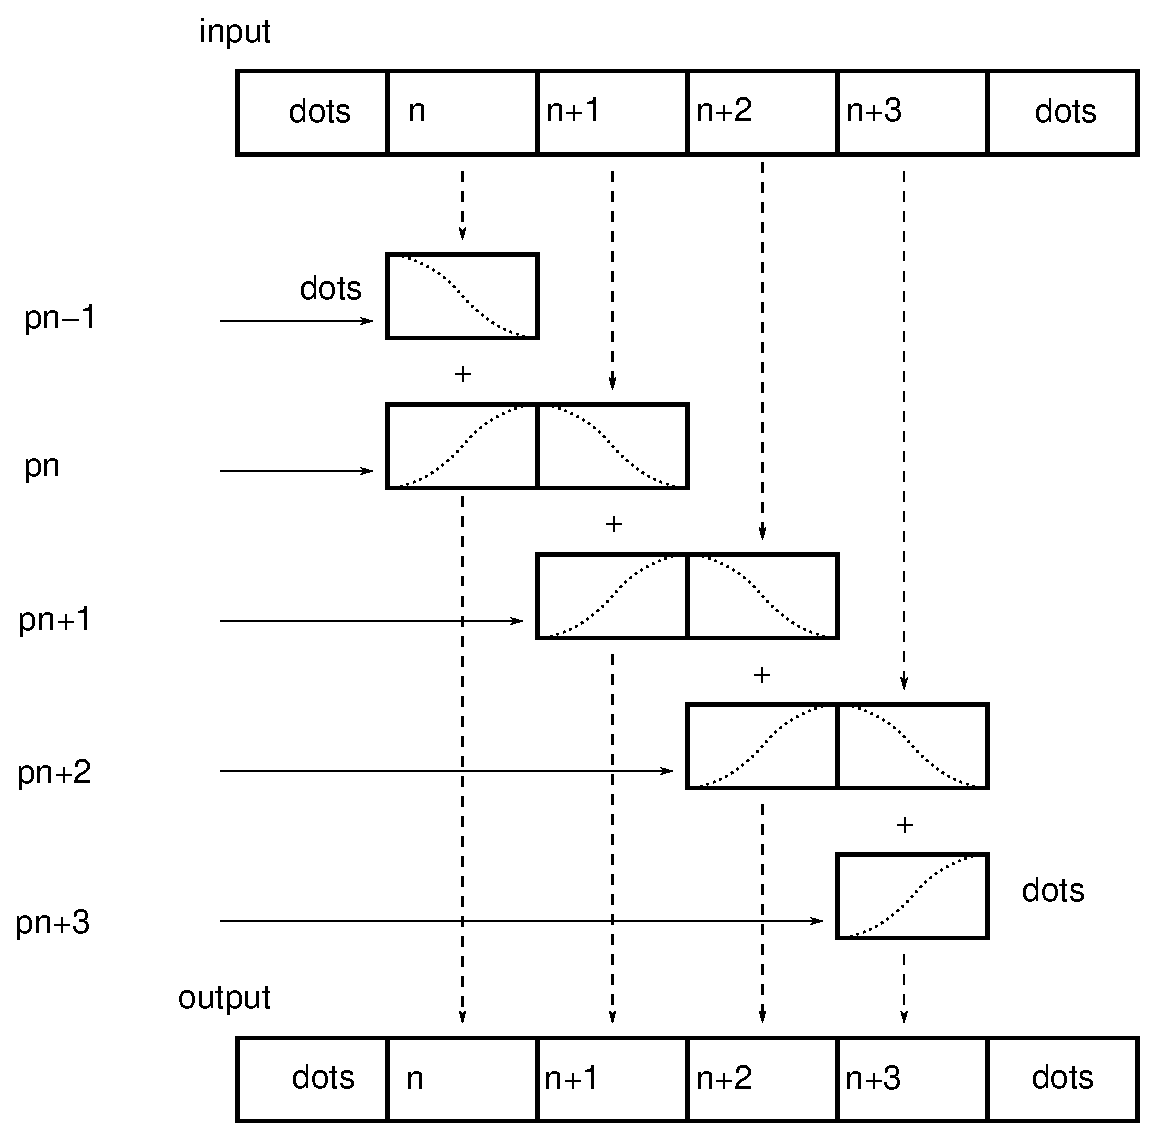
\includegraphics[width=.95\linewidth]{signal_processing}
\caption{\label{fig:signal_processing}{Illustration of the
frame-wise signal processing as implemented in the SSR renderers
(see text).}}
\end{figure}

The implementation approach described above is one version of the standard way
of implementing time-varying audio processing. Note however that this means
that with \emph{all} renderers, moving sources are not physically correctly
reproduced. The physically correct reproduction of moving virtual sources as in
\cite{Ahrens08:MOVING_AES,Ahrens08:SUPERSONIC_AES} requires a different
implementation approach which is computationally significantly more costly.

\subsection{Binaural Renderer}
\label{sec:binaural_renderer}

Binaural rendering is a technique where the acoustical influence of the human
head is electronically simulated to position virtual sound sources in space.
{\bf Be sure that you use headphones to listen.} Note that the current binaural
renderer reproduces all virtual sources exclusively as point sources.

The acoustical influence of the human head is coded in so-called head-related
impulse responses (HRIRs). The HRIRs are loaded from the file
\texttt{/usr/local/share/ssr/default\_hrirs.wav}. If you want to use different
HRIRs then use the \texttt{--hrirs=FILE} command line option or the SSR
configuration file (Section~\ref{sec:ssr_configuration_file}) to specify your
custom location. The SSR connects its outputs automatically to outputs 1 and 2
of your sound card.

For virtual sound sources which are closer to the reference position (= the
listener position) than 0.5 mtrs, the HRTFs are interpolated with a Dirac impulse. This
ensures a smooth transition of virtual sources from the outside of the
listener's head to the inside.

SSR uses HRIRs with an angular resolution of 1$^\circ$. Thus, the HRIR file
contains 720 impulse responses (360 for each ear) stored as a 720-channel
.wav-file. The HRIRs all have to be of equal length and have to be arranged in
the following order:
%
\begin{itemize}
\item[-] 1st channel: left ear, virtual source position 0$^\circ$
\item[-] 2nd channel: right ear, virtual source position 0$^\circ$
\item[-] 3rd channel: left ear, virtual source position 1$^\circ$
\item[-] 4th channel: right ear, virtual source position 1$^\circ$
\item[] \dots
\item[-] 720th channel: right ear, virtual source position 359$^\circ$
\end{itemize}
%
If your HRIRs have lower angular resolution you have to interpolate them to the
target resolution or use the same HRIR for serveral adjacent directions in
order to fulfill the format requirements. Higher resolution is not supported.
Make sure that the sampling rate of the HRIRs matches that of JACK. So far, we
know that both 16bit and 24bit word lengths work.

The SSR automatically loads and uses all HRIR coefficients it finds in the
specified file. You can use the \texttt{--hrir-size=VALUE} command line option in order
to limit the number of HRIR coefficients read and used to \texttt{VALUE}. You
don't need to worry if your specified HRIR length \texttt{VALUE} exceeds the
one stored in the file. You will receive a warning telling you what the score
is. The SSR will render the audio in any case.

The actual size of the HRIRs is not restricted (apart from processing power).
The SSR cuts them into partitions of size equal to the JACK frame buffer size and
zero-pads the last partition if necessary.

Note that there's some potential to optimize the performance of the SSR by
adjusting the JACK frame size and accordingly the number of partitions when a
specific number of HRIR taps are desired. The least computational load arises
when the audio frames have the same size like the HRIRs. By choosing shorter
frames and thus using partitioned convolution the system latency is reduced but
computational load is increased.

The HRIRs \texttt{impulse\_responses/hrirs/hrirs\_fabian.wav} we have included
in the SSR are HRIRs of 512 taps of the FABIAN mannequin~\cite{fabian} in an
anechoic environment. See the file \texttt{hrirs\_fabian\_documentation.pdf}
for details of the measurement.
%
\paragraph{Preparing HRIR sets}%
%
You can easily prepare your own HRIR sets for use with the SSR by adopting
the MATLAB \cite{matlab} script \texttt{data/matlab\_scripts/prepare\_hrirs\_kemar.m}
to your needs. This script converts the HRIRs of the KEMAR mannequin included
in the CIPIC database \cite{cipic} to the format which the SSR expects. See the script for
further information and how to obtain the raw HRIRs.


\subsection{\label{sec:brs}Binaural Room Synthesis Renderer}

The Binaural Room Synthesis (BRS) renderer is a binaural renderer (refer to
Section~\ref{sec:binaural_renderer}) which uses one dedicated HRIR set of each
individual sound source. The motivation is to have more realistic reproduction
than in simple binaural rendering. In this context HRIRs are typically referred
to as binaural room impulse responses (BRIRs).

Note that the BRS renderer does not consider any specification of a virtual
source's position. The positions of the virtual sources (including their
distance) are exclusively coded in the BRIRs. Consequently, the BRS renderer
does not apply any distance attenuation. It only applies the respective
source's gain and the master volume. No interpolation with a Dirac as in the
binaural renderer is performed for very close virtual sources. The only
quantity which is explicitely considered is the orientation of the receiver,
i.e.~the reference. Therefore, specification of meaningful source and receiver
positions is only necessary when a correct graphical illustration is desired.

The BRIRs are stored in the a format similar to the one for the HRIRs for the
binaural renderer (refer to Section~\ref{sec:binaural_renderer}). However,
there is a fundamental difference: In order to be consequent, the different
channels do not hold the data for different positions of the virtual sound
source but they hold the information for different head orientations.
Explicitely,
%
\begin{itemize}
\item[-] 1st channel: left ear, head orientation 0$^\circ$
\item[-] 2nd channel: right ear, head orientation 0$^\circ$
\item[-] 3rd channel: left ear, head orientation 1$^\circ$
\item[-] 4th channel: right ear, head orientation 1$^\circ$
\item[] \dots
\item[-] 720th channel: right ear, head orientation 359$^\circ$
\end{itemize}
%
In order to assign a set of BRIRs to a given sound source an appropriate scene
description in \texttt{.asd}-format has to be prepared (refer also to
Section~\ref{sec:audio_scenes}). As shown in \texttt{brs\_example.asd} (from
the example scenes), a virtual source has the optional property
\texttt{properties\_file} which holds the location of the file containing the
desired BRIR set. The location to be specified is relative to the folder of the
scene file. Note that -- as described above -- specification of the virtual
source's position does not affect the audio processing. If you do not specify a
BRIR set for each virtual source, then the renderer will complain and refuse
processing the respective source.

We have measured the binaural room impulse responses of the FABIAN
mannequin~\cite{fabian} in one of our mid-size meeting rooms called Sputnik
with 8 different source positions. Due to the file size, we have not included
them in the release. Please contact \contactadress\ to obtain the data.


%\subsection{Binaural Playback Renderer}
%
%The binaural playback (BPB) renderer is actually not a renderer but
%a playback engine that enables real-time head-tracking in headphone
%playback. It is similar to BRS with the only difference that it does
%not employ impulse responses that are applied to the input signal.
%It is rather such that the entire signals for the two ears for all
%desired possible head orientations have to be precomputed and are then
%loaded into the memory. During playback, depending on the
%instantaneous head orientation of the listener as measured by the
%tracking system, the corresponding audio data are replayed. If a
%change in head orientation occurs then a crossfade is applied over
%the duration of one JACK frame. Playing is automatically looped. To
%stop replay, mute the source. When the source is unmuted, replay
%starts at the beginning of the data.
%
%The BPB renderer was designed for the simulation of time-varying
%systems, which are complicated to implement in real-time. The
%audio signals can be prepared in any desired software and also
%costly algorithms that do not run in real-time can be replayed with
%head-tracking.
%
%As shown in the example \texttt{bin/scenes/bpb\_example.asd} and
%similar to the description of a BRS scene, a virtual source has the
%optional property \texttt{properties\_file}, which holds the location
%of the file containing the audio data. By default, it is assumed
%that the data are stored in a 720-channel audio file the channels of
%which are arranged similarly to BRS impulse responses.
%
%Loading all 720 channels into memory can result in hundreds of
%megabytes even for signals of moderate length. In order to avoid
%restrictions due to the available memory caused by possibly unrequired 
%data it is possible to restrict the interval of head
%orientations. This restriction has to be applied symmetrically,
%e.g.~$\pm60^\circ$. The resolution between the limits is still
%1$^\circ$. The channel arrangement for the $\pm60^\circ$ example
%would then be
%%
%\begin{itemize}
%\item[-] 1st channel: left ear, head orientation 0$^\circ$
%\item[-] 2nd channel: right ear, head orientation 0$^\circ$
%\item[-] 3rd channel: left ear, head orientation 1$^\circ$
%\item[-] 4th channel: right ear, head orientation 1$^\circ$
%\item[] \dots
%\item[-] 121st channel: left ear, head orientation 60$^\circ$
%\item[-] 122nd channel: right ear, head orientation 60$^\circ$
%\item[-] 123rd channel: left ear, head orientation 300$^\circ$ (i.e.~-60$^\circ$)
%\item[-] 124th channel: right ear, head orientation 300$^\circ$ (i.e.~-60$^\circ$)
%\item[-] 125th channel: left ear, head orientation 301$^\circ$ (i.e.~-59$^\circ$)
%\item[-] 126th channel: right ear, head orientation 301$^\circ$ (i.e.~-59$^\circ$)
%\item[] \dots
%\item[-] 242nd channel: right ear, head orientation 359$^\circ$ (i.e.~-1$^ \circ$)
%\end{itemize}
%%
%resulting thus in 242 channels. It is not necessary to explicitly
%specify the desired interval of possible head orientations. The SSR deduces it 
%directly from the number of channels of the
%\texttt{properties\_file}. If the listener turns the head to
%orientations for which no data are available the BPB renderer
%automatically replays the data for the closest orientation available.
%We assume that this is less disturbing in practice than a full
%dropout of the signal.
%
%To fulfill the ASDF syntax, the specification of an input signal is
%required. In order to avoid the unnecessary opening and replaying of
%an audio file, we propose to specify an arbitrary input port such as
%
%\begin{verbatim}
%<source name="source" properties_file="../audio/binaural_data.wav">
%  <!-- this is arbitrary -->
%  <port>0</port>
%  <!-- this only influences the GUI -->
%  <position x="-2" y="2"/>
%</source>
%\end{verbatim}

\subsection{Vector Base Amplitude Panning Renderer}

The Vector Base Amplitude Panning (VBAP) renderer uses
the algorithm described in
\cite{Pulkki97:JAES}. It tries to find a loudspeaker pair between
which the phantom source is located (in VBAP you speak of a phantom
source rather than a virtual one). If it does find a loudspeaker pair
whose angle is smaller than $180^\circ$ then it calculates the weights
$g_l$ and $g_r$ for
the left and right loudspeaker as
%
\begin{equation}
g_{l,r} = \frac{\cos\phi \sin \phi_0 \pm \sin \phi \cos \phi_0}
{2\cos \phi_0 \sin \phi_0} \ . \nonumber
\end{equation}
%
$\phi_0$ is half the angle between the two loudspeakers with respect to the
listening position, $\phi$ is the angle between the position of the phantom
source and the direction ``between the loudspeakers''.

If the VBAP renderer can not find a loudspeaker pair whose angle is smaller
than $180^\circ$ then it uses the closest loudspeaker provided that the latter
is situated within $30^\circ$. If not, then it does not render the source. If
you are in verbosity level 2 (i.e.~start the SSR with the \texttt{-vv} option)
you'll see a notification about what's happening.

Note that all virtual source types (i.e.~point and plane sources) are rendered
as phantom sources.

Contrary to WFS, non-uniform distributions of loudspeakers are ok here.
Ideally, the loudspeakers should be placed on a circle around the reference
position. You can optionally specify a delay for each loudspeakers in order to
compensate some amount of misplacement. In the ASDF (refer to
Section~\ref{sec:asdf}), each loudspeaker has the optional attribute
\texttt{delay} which determines the delay in seconds to be applied to the
respective loudspeaker. Note that the specified delay will be rounded to an
integer factor of the temporal sampling period. With 44.1 kHz sampling
frequency this corresponds to an accuracy of 22.676 $\mu$s, respectively an
accuracy of 7.78 mm in terms of loudspeaker placement. Additionally, you can
specify a weight for each loudspeaker in order to compensate for irregular
setups. In the ASDF format (refer to Section~\ref{sec:asdf}), each loudspeaker
has the optional attribute \texttt{weight} which determines the linear~(!)
weight to be applied to the respective loudspeaker. An example would be
%
\begin{verbatim}
<loudspeaker delay="0.005" weight="1.1">
        <position x="1.0" y="-2.0"/>
        <orientation azimuth="-30"/>
</loudspeaker>
\end{verbatim}
%
Delay defaults to 0 if not specified, weight defaults to~1.

Although principally suitable, we do not recommend to use our amplitude panning
algorithm for dedicated 5.1 (or comparable) mixdowns. Our VBAP renderer only
uses adjacent loudspeaker pairs for panning which does not exploit all
potentials of such a loudspeaker setup. For the mentioned formats specialized
panning processes have been developed also employing non-adjacent loudspeaker
pairs if desired.

The VBAP renderer is rather meant to be used with non-standardized setups.
%
\subsection{Wave Field Synthesis Renderer}

The Wave Field Synthesis (WFS) renderer is the only renderer so far which
discriminates between virtual point sources and plane waves. It implements the
simple driving function given in~\cite{Spors08:WFS_AES}. Note that we have only
implemented a temporary solution to reduce artifacts when virtual sound sources
are moved. This topic is subject to ongoing research. We will work on that in
the future. In the SSR configuration file
(Section~\ref{sec:ssr_configuration_file}) you can specify an overall predelay
(this is necessary to render focused sources) and the overall length of the
involved delay lines. Both values are given in samples.

%
\paragraph{Prefiltering}%
%
As you might know, WFS requires a spectral correction additionally to the delay
and weighting of the input signal. Since this spectral correction is equal for
all loudspeakers, it needs to be performed only once on the input. We are
working on an automatic generation of the required filter. Until then, we load
the impulse response of the desired filter from a .wav-file which is specified
via the \texttt{--prefilter=FILE} command line option (see
Section~\ref{sec:running_ssr}) or in the SSR configuration file
(Section~\ref{sec:ssr_configuration_file}). Make sure that the specified audio
file contains only one channel. Files with a differing number of channels will
not be loaded. Of course, the sampling rate of the file also has to match that
of the JACK server.

Note that the filter will be zero-padded to the next highest power of 2. If the
resulting filter is then shorter than the current JACK frame size, each
incoming audio frame will be divided into subframes for prefiltering. That
means, if you load a filter of 100 taps and JACK frame size is 1024, the filter
will be padded to 128 taps and prefiltering will be done in 8 cycles. This is
done in order to save processing power since typical prefilters are much
shorter than typical JACK frame sizes. Zero-padding the prefilter to the JACK
frame size usually produces large overhead. If the prefilter is longer than the
JACK frame buffer size, the filter will be divided into partitions whose length
is equal to the JACK frame buffer size.

If you do not specify a filter, then no prefiltering is performed. This results
in a boost of bass frequencies in the reproduced sound field.

In order to assist you in the design of an appropriate prefilter, we have
included the MATLAB \cite{matlab} script
\texttt{data/matlab\_scripts/make\_wfs\_prefilter.m} which does the job. In the
very top of the file, you can specify the sampling frequency, the desired
length of the filter as well as the lower and upper frequency limits of the
spectral correction. The lower limit should be chosen such that the subwoofer
of your system receives a signal which is not spectrally altered. This is due
to the fact that only loudspeakers which are part of an array of loudspeakers
need to be corrected. The lower limit is typically around 100 Hz. The upper
limit is given by the spatial aliasing frequency. The spatial aliasing is
dependent on the mutual distance of the loudspeakers, the distance of the
considered listening position to the loudspeakers, and the array geometry. See
\cite{Spors06:Aliasing_AES} for detailed information on how to determine the
spatial aliasing frequency of a given loudspeaker setup. The spatial aliasing
frequency is typically between 1000 Hz and 2000 Hz. For a theoretical treatment
of WFS in general and also the prefiltering, see \cite{Spors08:WFS_AES}.

The script \texttt{make\_wfs\_prefilter.m} will save the impulse response of
the designed filter in a file like
\texttt{wfs\_prefilter\_120\_1500\_44100.wav}. From the file name you can
extract that the spectral correction starts at 120 Hz and goes up to 1500 Hz at
a sampling frequency of 44100 Hz. Check the folder
\texttt{data/impules\_responses/wfs\_prefilters} for a small selection of
prefilters.
%
\paragraph{Tapering}%
%
When the listening area is not enclosed by the loudspeaker setup, artifacts
arise in the reproduced sound field due to the limited aperture. This problem
of spatial truncation can be reduced by so-called tapering. Tapering is
essentially an attenuation of the loudspeakers towards the ends of the setup.
As a consequence, the boundaries of the aperture become smoother which reduces
the artifacts. Of course, no benefit comes without a cost. In this case the
cost is amplitude errors for which the human ear fortunately does not seem to
be too sensitive.

In order to taper, you can assign the optional attribute \texttt{weight} to
each loudspeaker in ASDF format (refer to Section~\ref{sec:asdf}). The
\texttt{weight} determines the linear~(!) weight to be applied to the
respective loudspeaker. It defaults to 1 if it is not specified.


\subsection{Ambisonics Amplitude Panning Renderer}

The Ambisonics Amplitude Panning (AAP) renderer does very simple Ambisonics
rendering. It does amplitude panning by simultaneously using all loudspeakers
which are not subwoofers to reproduce a virtual source (contrary to the VBAP
renderer which uses only two loudspeakers at a time). Note that the
loudspeakers should ideally be arranged on a circle and the reference should be
the center of the circle. The renderer checks for that and applies delays and
amplitude corrections to all loudspeakers which are closer to the reference
than the farthest. This also includes subwoofers. If you do not want close
loudspeakers to be delayed, then simply specify their location in the same
direction like its actual position but at a larger distance from the reference.
Then the graphical illustration will not be perfectly aligned with the real
setup, but the audio processing will take place as intended. Note that the AAP
renderer ignores delays assigned to an individual loudspeaker in ASDF. On the
other hand, it does consider weights assigned to the loudspeakers. This allows
you to compensate for irregular loudspeaker placement.

Note finally that AAP does not allow to encode the distance of a virtual sound
source since it is a simple panning renderer. All sources will appear at the
distance of the loudspeakers.

If you do not explicitly specify an Ambisonics order, then the maximum order
which makes sense on the given loudspeaker setup will be used. The
automatically chosen order will be one of \nicefrac{(L-1)}{2} for an odd number
$L$ of loudspeakers and accordingly for even numbers.

You can manually set the order via a command line option
(Section~\ref{sec:running_ssr}) or the SSR configuration file
(Section~\ref{sec:ssr_configuration_file}). We therefore do not explicitly
discriminate between ``higher order'' and ``lower order'' Ambisonics since this
is not a fundamental property. And where does ``lower order'' end and ``higher
order'' start anyway?

Note that the graphical user interface will not indicate the activity of the
loudspeakers since theoretically all loudspeakers contribute to the sound field
of a virtual source at any time.

\paragraph{Conventional driving function}

By default we use the standard Ambisonics panning function outlined e.g.~in
\cite{Neukom07} reading
%
\begin{equation}
d(\alpha_0)  = \frac{\sin\left ( \frac{2M+1}{2} \ (\alpha_0 -
\alpha_\textnormal{s})\right )} {(2M+1) \ \sin \left ( \frac{\alpha_0 -
\alpha_\textnormal{s}}{2} \right ) } \ , \nonumber
\end{equation}
%
whereby $\alpha_0$ is the polar angle of the position of the considered secondary source,
$\alpha_\textnormal{s}$ is the polar angle of the position of the virtual source, and
$M$ is the Ambisonics order.

\paragraph{In-phase driving function}

The conventional driving function leads to both positive and negative weights
for individual loudspeakers. An object (e.g.~a listener) introduced into the
listening area can lead to an imperfect interference of the wave fields of the
individual loudspeakers and therefore to an inconsistent perception.
Furthermore, conventional Ambisonics panning can lead to audible artifacts for
fast source motions since it can happen that the weights of two adjacent audio
frames have a different algebraic sign.

These problems can be worked around when only positive weights are applied on
the input signal (\emph{in-phase} rendering). This can be accomplished via the
in-phase driving function given e.g.~in \cite{Neukom07} reading
%
\begin{equation}
d(\alpha_0) = \cos^{2M} \left (\frac{\alpha_0 - \alpha_\textnormal{s}}{2} \right ) \ . \nonumber
\end{equation}
%
Note that in-phase rendering leads to a less precise localization of the virtual source
and other unwanted perceptions. You can enable in-phase rendering via the according command-line
option or you can set
the \texttt{IN\_PHASE\_RENDERING} property in the SSR configuration file (see section~\ref{sec:ssr_configuration_file}) to be ``\texttt{TRUE}'' or ``\texttt{true}''.

\subsection{Generic Renderer}

The generic renderer turns the SSR into a multiple-input-multiple-output
convolution engine. You have to use an ASDF file in which the attribute
\texttt{properties\_file} of the individual sound source has to be set
properly. That means that the indicated file has to be a multichannel file with
the same number of channels like loudspeakers in the setup. The impulse
response in the file at channel 1 represents the driving function for
loudspeaker~1 and so on.

Be sure that you load a reproduction setup with the corresponding number of
loudspeakers.

It is obviously not possible to move virtual sound sources since the loaded
impulse responses are static. We use this renderer in order to test advanced
methods before implementing them in real-time or to compare two different
rendering methods by having one sound source in one method and another sound
source in the other method.

Download the ASDF examples from~\cite{ssr} and check out the file
\texttt{generic\_renderer\_example.asd} which comes with all required data.

\begin{table}%[htbp]
\begin{center}
\begin{tabular}{| l | c | c |}
\hline
 & individual delay & weight \\
 \hline
 binaural renderer & - & - \\
 BRS renderer & - & - \\
 VBAP renderer & + & + \\
 WFS renderer & - & + \\
 AAP renderer & autom. & + \\
 generic renderer & - & - \\\hline
\end{tabular}
\caption{\label{tab:loudspeaker_properties}Loudspeaker properties
considered by the different renderers.}
\end{center}
\end{table}

\begin{table}%[htbp]
\begin{center}%
\begin{minipage}{\textwidth}% to enable footnotes
\begin{tabular}{| l | c | c | c | c | c |}
\hline
      & gain & mute & position & orientation\footnote{So far, only plane waves have a defined
orientation.} & model\\
                    \hline
 binaural renderer & + & + & + & - & only ampl.\\
 BRS renderer      & + & + & - & - & -\\
 VBAP renderer     & + & + & + & - & only ampl.\\
 WFS renderer      & + & + & + & + & +\\
 AAP renderer      & + & + & + & - & only ampl.\\
 generic renderer  & + & + & - & - & -\\\hline
\end{tabular}
\end{minipage}
\caption{\label{tab:source_properties}Virtual source's properties
considered by the different renderers.}
\end{center}
\end{table}


%\subsection{Parallel Processing Renderers}
%
%The renderers as described above do not support parallel processing. We are
%currently redesigning the architecture of the SSR in order to support audio
%processing in multiple threads so that the power of multi-processor/multi-core machines can be
%properly exploited. The current SSR release contains versions of the WFS, the
%VBAP, and the binaural renderer which support parallel processing. These
%versions are disabled at compile time by default.
%If you want to enable these renderers use the option \texttt{./configure
%--enable-newrenderer} (Section~\ref{sec:comp_inst}) when configuring. All
%renderers other than WFS, VBAP, and binaural will then not be available.
%
%\textbf{WARNING:} The parallel processing renderers are under heavy development.
%If you encounter unexpected behaviour or bugs, please report them to 
%\emph{SoundScapeRenderer@telekom.de}. Thank you. 

\subsection{Summary}

Tables~\ref{tab:loudspeaker_properties}
and~\ref{tab:source_properties} summarize the functionality of the
SSR renderers.


\section{Graphical User Interface}
\label{sec:gui}
%
Our graphical user interface (GUI) is quite costly in terms of
computation. So we emphatically recommend that you {\bf properly
configure the hardware acceleration of your graphics card}.
If you still have performance
issues make the window as small as possible. The smaller
the window is the less is the processing cost.

The SSR GUI tries to enable samplebuffer support to enable
anti-aliasing of the screen output. It will tell you if it didn't
work out. Check Fig.~\ref{fig:anti_aliasing} to get an idea of
the influence of anti-aliasing.
%
One day we will also implement a variable frequency for the
screen update so that you can slow it down if CPU load is too high. Of course it
won't look as nice then.

\begin{figure}[htbp]
\begin{center}
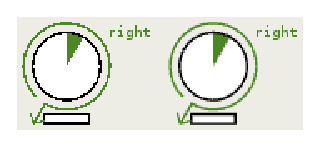
\includegraphics[scale=1]{anti_aliasing}
\caption{\label{fig:anti_aliasing}{No anti-aliasing on the left image.}}
\end{center}
\end{figure}

\begin{figure}[!t]% place the figure on top of the page
\begin{center}
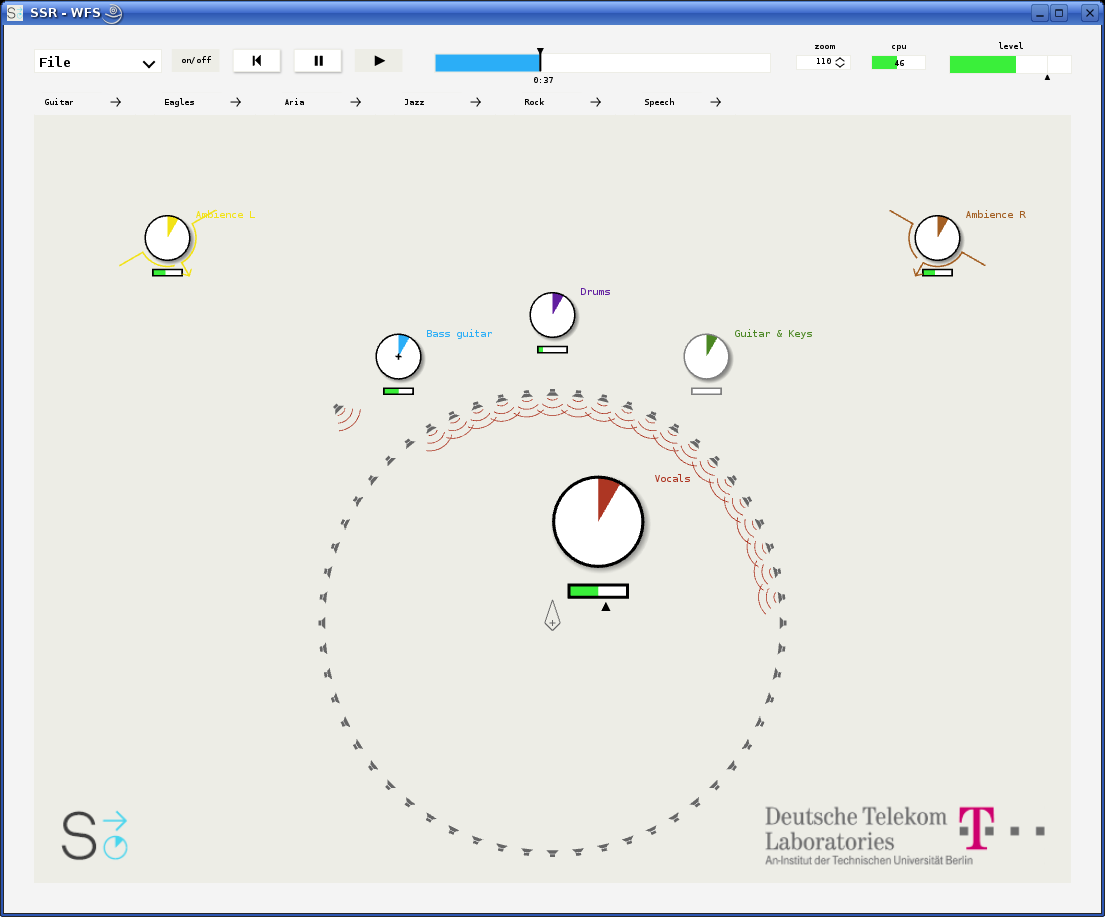
\includegraphics[width=\linewidth]{screenshot}
\caption{\label{fig:screenshot}{Screen shot of the SSR GUI.
%The current
%loudspeaker setup is a ring of 56 loudspeakers plus a subwoofer. In this case,
%WFS rendering was chosen. Both ``Ambiance'' sources emit plane waves, all
%other sources are point sources. Source ``Vocals'' is selected and the corresponding
%loudspeaker activity is indicated. Source ``Bass guitar'' is static and source
%``Guitar \& Keys'' is muted.
}}
\end{center}
\end{figure}
%
\subsection{General Layout}

The graphical user interface (GUI) consists mainly of an
illustration of the scene that you are hearing and some interaction
tools. The renderer type is indicated in the window title.
See a screen shot in Fig.~\ref{fig:screenshot}.

On the top left you will find the file menu where you can open files, save
scenes, and quit the application. So far only the \emph{save scene as\dots}
option is available. That means every time to save the current scene you will
be asked to specify the file name. This will be made more convenient in the
future.

Next to the file menu, there is a button which lets you activate and deactivate
the audio processing. Deactivating the audio processing does not necessarily
lower the CPU load. It means rather that the SSR won't give any audio output,
neither for involved audio files nor for live inputs.

Next to the processing button, you find the transport section with buttons to
skip back to the beginning of a scene, pause replaying, and continue/start
playing. Note that pausing a scene does not prevent live inputs from being
processed. To prevent audio output switch off processing (see above). You may
also replay while processing is switched off to navigate to a certain point in
time in the respective scene.

In the top middle section of the GUI there is the audio scene time line.
By default, it shows a time interval of two minutes duration. Whenever
the progress exceeds the displayed time interval the latter is shifted
such that the progress is always properly indicated.
Below the handle, there is a numerical
indication of the elapsed time with respect to the beginning of the scene.
See Sec.~\ref{sec:mouse_actions}
for information on how to operate on the time line.

To the right of the time line there's the CPU load gauge. It
displays the average CPU load as estimated by the JACK audio
server on a block-wise basis.
Further right there's the label to indicate the current zoom factor
in percent.

And finally, on the top right you find the master level meter combined with the
master volume fader. The colored bar indicates an estimation of the relative
maximum audio level in dB, also updated block-wise. The left boundary of the
meter is at -50~dB; the right boundary is at +12~dB. The black triangle below
the colored bar indicates the master volume in dB. Click somewhere into the
widget and the master volume gets additionally displayed as a number. Note that
this meter displays full scale, i.e.~above 0~dB clipping and thus distortion of
the output signal occurs! 0~dB is indicated by a thin vertical line.

In the row below the transport section, you occasionally find some tabs giving
fast access to a number of scenes. These tabs can be defined in a file. By 
default, the file \texttt{scene\_menu.conf} in the current working directory is
assumed; there is also an option to specify the file name in the SSR 
configuration file. Refer to Sec.~\ref{sec:ssr_configuration_file}. The 
configuration file for the tabs may contain something like the following:
%
\begin{verbatim}
# This file configures the menu for the scene selection.
#
scenes/dual_mono.asd Guitar######### comments are possible
scenes/jazz.asd Jazz
scenes/rock.asd Rock
#scenes/speech.asd Speech
scenes/live_conference.xml live conference
\end{verbatim}
%
The syntax is as follows:
\begin{itemize}
\item[-] Everything after a hash symbol (\#) in a line is ignored.
\item[-] A valid entry consists of the path (relative or absolute)
to ASDF file (or pure audio file) followed by space and a short
keyword that will be displayed on the respective tab on the screen.
\end{itemize}
%
Of course, also audio files can be specified instead of \texttt{.asd}s. Note
that so far, no syntax validation is performed, so watch your typing. We
furthermore recommend that you keep the keywords short because space on the
screen is limited. Note also that only those tabs are displayed which fit on
the screen.

The SSR always tries to find the file \texttt{scene\_menu.conf} in its current
working directory (or at the location specified in the SSR configuration file). 
If is does not find it no tabs will be displayed in the GUI.
So you can have several of such files at different locations. We have added an
example in folder \texttt{data/}.

The main part of the screen is occupied by the graphical
illustration of the scene that you are hearing. The orientation of the coordinate
system is exactly like depicted in Fig.~\ref{fig:coordinate_system}.
I.e., the $x$-axis points to the right of the screen, the $y$-axis points to the top
of the screen. The origin of the coordinate system is marked by a cross, the reference
is marked by a rhomb. The direction ``straight in front'' is typically assumed to be
vertically upwards on the screen, especially for binaural techniques. We do so as well.
Note that in this case ``straight in front'' means $\alpha = 90^\circ$ and NOT
$\alpha=0^\circ$.

In Fig.~\ref{fig:screenshot} you see a number of sound sources with their
individual audio level meters (combined with their individual volume
sliders) underneath. The left hand boundary of the level meter is at -50~dB; the right
hand boundary is at 0~dB. Spherical sources don't have any additional
decoration. The wave front and propagation direction of plane waves
are indicated.

You also see icons for the loudspeakers of the current rendering
setup (if the currently applied technique employs any).
%In 
%Fig.~\ref{fig:screenshot} you see the system that is installed in our
%Usability laboratory. It is a ring of a diameter of a bad 3
%meters hosting 56 equiangularly spaced loudspeakers plus a subwoofer.
%
%The rhombus inside the loudspeaker ring
%indicates the location and orientation of the reference point of the
%current setup.

\subsection{Mouse Actions}
\label{sec:mouse_actions}

The GUI is designed such that the most important functionalities
can be accessed via a touch screen. Thus, it mostly employs 'left
clicks' with the mouse.

The use of the file and transport section is rather intuitive so we
won't further explain it here. The time line can be used to jump to
a certain position within the sound scene and it also shows the
progress of the scene. Click into the white/blue area of the time
line in order to jump to a specific point in time, or drag the
handle to fast forward or rewind. Left-clicking to the right of the
time line skips forward by 5 seconds, left-clicking to the left of
the time line skips back by 5 seconds. Double-clicking on the time
line skips back to the beginning of the scene. Right-clicking on the
time line opens an input window in order that you can numerically
specify the time instant to jump to (refer to
Sec.~\ref{sec:keyboard_actions}).

You can change the zoom either by clicking into the zoom label and
dragging up or down for zooming in or out. Alternatively, you can use the
mouse wheel.
Clicking and dragging on the background of the screen lets you move
inside the scene. A double-click brings you back to the default
position and also defaults the zoom.

Clicking and dragging on a sound source lets you select and move it. Note that
you cannot directly manipulate the propagation direction of plane waves. It's
rather such that plane sources always face the reference point. To change their
direction of incidence move the plane wave's origin point to the appropriate 
position. Right clicking on a sound source opens a window which lists the 
properties of the source such as position, volume, etc. Refer to 
Fig.~\ref{fig:screenshot_spd} and Sec.~\ref{sec:source_properties_dialog}.

A right mouse click on the scene background lets you select multiple
sound sources via a rubber band.

If you hold the \texttt{Ctrl} key pressed during any mouse action then you
operate on all selected sound sources at the same time (i.e.~mute,
move, etc.~them).

Click on the SSR logo and you'll see the \emph{About the SSR}
information.

\subsubsection{Source Properties Dialog}
\label{sec:source_properties_dialog}

\begin{figure}
\begin{center}
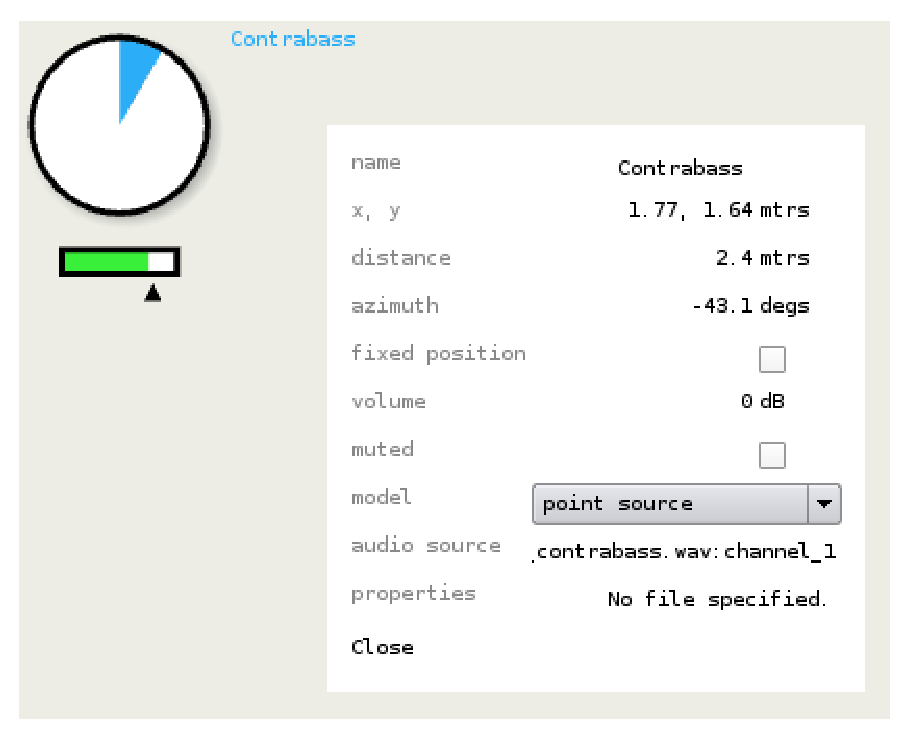
\includegraphics[scale=0.4]{screenshot_spd}
\caption{\label{fig:screenshot_spd}{Source properties dialog}}
\end{center}
\end{figure}

The source properties dialog can be accessed via a right click on a source and 
shows information about the actual state of the selected source. Its main 
purpose is to provide the possibility of an exact positioning of sources. The 
properties \texttt{fixed position}, \texttt{muted} and \texttt{model} can be 
changed. Please refer to figure \ref{fig:screenshot_spd} to see the complete 
list of properties this dialog shows. 

\subsection{Keyboard Actions}
\label{sec:keyboard_actions}
%
A number of keyboard actions have been implemented as listed below. Recall that also
some keyboard actions are available when the SSR is run without GUI (refer to 
Sec.~\ref{sec:running_ssr}).
%
\begin{itemize}
\item[] \texttt{+/-}: if no sound source is selected: raise/lower master volume by 1dB,\\
  otherwise raise/lower the selected sources' volume by 1dB
\item[] \texttt{Arrow up/down/left/right}: navigate in scene
\item[] \texttt{Space}: toggles the play/pause state
\item[] \texttt{Backspace}: skip to beginning of scene
\item[] \texttt{Return}: calibrate tracker (if present). When pressed, the instantaneous\\
  orientation is assumed to be straight forward (i.e.~90$^\circ$ azimuth)
\item[] \texttt{Ctrl}: when pressed, multiple sound sources can be
selected via mouse clicks or operations can be performed on multiple sources simultaniously
\item[] \texttt{Ctrl+Alt}: individual sound sources can be
deselected from a larger selection via a mouse click or the rubber band
\item[] \texttt{Ctrl+a}: select all sources
\item[] \texttt{f}: toggles the position-fix-state of all selected sound sources (sources
  which can not be moved are marked with a little cross)
\item[] \texttt{m}: toggles the mute state of all selected sound sources (muted sources
  are displayed with a grey frame instead of a black one)
\item[] \texttt{p}: toggles the source model between \emph{plane wave} and \emph{point source}
\item[] \texttt{s}: if no source selected: unsolos all potentially soloed sources,\\
  otherwise: solos selected sound sources.
\item[] \texttt{Ctrl+s}: opens the \emph{save scene as\dots} dialog
\item[] \texttt{F11}: toggles window fullscreen state
\item[] \texttt{1-9}: select source no.~1-9
\item[] \texttt{0}: deselect all sources
\item[] \texttt{Ctrl+c}: quit
\item[] \texttt{Ctrl+t}: open text edit for time line. The format is
\texttt{hours:mins(2digits):secs(2digits)} whereby \texttt{hours:}
and \texttt{hours:mins(2digits):} can be omitted if desired.
\item[] \texttt{Esc}: quit
\end{itemize}
%
%
%

% This is the section about the network interface.
% It is included by SoundScapeRenderer.tex

\section{Network Interface}
\label{sec:network}

This is just a short overview about the XML messages which can be sent to the
SSR via TCP/IP.
The messages have to be terminated with a binary zero (\verb|\0|).

\textbf{WARNING:} We
did not evaluate the network interface in terms of security. So please be sure
that you are in a safe network when using it.

% The SSR provides a network interface to enable a remote control of the audio
% processing part. A typical usage could be to dynamically modify a sound scene
% using any kind of interaction tool. This interaction tool (e.g. a head-tracker)
% then communicates with the SSR via the SSR's network interface.

% \begin{figure}
% %\vspace{0.3cm}
% \begin{center}
% \includegraphics[width=\textwidth]{ssrsystem}
% %\vspace{-2.0cm}
% \caption{\label{fig:ssrsystem}{The SoundScape Renderer Build.}}
% \end{center}
% %\vspace{-0.7cm}
% \end{figure}

% \subsection{General Layout}
%
% The network server is connected to the main component of the SSR which is the audio
% processing part. The server communicates with its clients such as GUIs or trackers
% and transfers the received data to the core part of the SSR. Note that the
% communication is bidirectional, i.e. clients can also receive messages from the
% server.\\
% The basic server thread initializes the network socket and waits for an incomming connection.
% When a new client joins the server, the server starts the handling routines. These handling
% routines are splitted into two seperate threads, one for receiving, the other for sending data.
% Like this, it is possible to receive and send at the same
% time.\\
% Prepared but not finished are file handling routines, so that e.g. a sound file on the audio
% processing computer can be opened from a remote GUI. The (intended) functinoality is comparable
% to that of an ftp server.\\
% The network protocol is TCP/IP. The data transport is in plaintext. The application protocol
% is a simpler format than the ftp protokoll. Messages begin with a code number followed by the
% payload.\\
% The complete client-server-communication flow is shown in figure \ref{fig:networkflow}.

% \begin{figure}
% %\vspace{0.3cm}
% \begin{center}
% \includegraphics[width=\textwidth]{networkflow}
% %\vspace{-2.0cm}
% \caption{\label{fig:networkflow}{Network Subsystem.}}
% \end{center}
% %\vspace{-0.7cm}
% \end{figure}

% \subsection{Class Description}
% %
% \subsubsection{Files}
% %
% All the network related source files are stored in the folder \texttt{src/network} (see table \ref{tab:network_files}).
% %
% \begin{table}
% \begin{center}
% \begin{tabular}{ll}
% \hline
% \textsc{Name} & \textsc{Description} \\
% \hline%\hline
% Client.cpp & Client class implementation\\
% %   \hline
% Client.h & Client class declaration\\
% %   \hline
% ClientConfigFile.cpp & config-file parser for client\\
% %   \hline
% FileHandle.cpp & File handling routines for using like ftp\\
% %   \hline
% FileHandle.h & Class declaration\\
% %   \hline
% NetworkInterface.cpp & SSR Server Network Interface\\
% %   \hline
% NetworkInterface.h & Interface declaration\\
% %   \hline
% ParseXMLCommand.cpp & XML-String Parser for Server and Client\\
% %   \hline
% ParseXMLCommand.h & XML Parser declaration\\
% %   \hline
% RequestHandle.cpp & Client request handling at server side\\
% %   \hline
% RequestHandle.h & Class declaration\\
% %   \hline
% SSRClientNetworkInterface.cpp & SSR Client Network Interface\\
% %   \hline
% SSRClientNetworkInterface.h & Classe declaration\\
% %   \hline
% Server.cpp & SSR Server routines\\
% %   \hline
% Server.h & Class declaration\\
% %   \hline
% Socket.cpp & Fundamental Network routines\\
% %   \hline
% Socket.h & Class declaration\\
% %   \hline
% server\_codes.h & Server Codes for Messages\\
% \hline
% \end{tabular}
% \label{tab:network_files}
% \end{center}
% \caption{Source files in folder \texttt{src/network}}
% \end{table}
% %
% %
% \subsubsection{Class ``Socket''}
% %
% This is the fundamental network class. It provides the functions to initialize the network,
% requesting, binding, connecting and closing sockets. For further information, confer to the header file
% \texttt{src/nework/Socket.h}.
% %
% %
% \subsubsection{Class ``Server''}
% %
% The Server class is derived from the socket class. The Server is written for running standalone. It
% can thus easily be reused in other projects. The initialization function expects four
% optional arguments at startup. These are
% %
% \begin{enumerate}
%     \item Server Name
%   \item Network Port
%   \item IP-Address
%   \item XML File Directory
% \end{enumerate}
% %
% The Server Name is a string which is send to each client when it joins. This is usefull
% for the client to identify the server and see that the connection is established.\\
% The Network Port specifies the network port on which server listens for incomming messages.\\
% With the IP-Address option, it is possible to bind the server to one specific IP-Address. If
% no IP-address is specified, the server listens on all network cards respectively IP-addresses.\\
% Finally, the XML File Directory is not yet in use.\\
% Note that all parameters are optional. When a parameter is not specified, default value are used.
% These are defined in the header file \texttt{src/network/Server.h}. A client data structure is
% also defined in the header. This structure contains status information about the clients.\\
%
% The main thread looks for incomming clients, sets the client structure
% and starts the client request handling via a callback function. Upon successful connection, it stores the client object
% in a list. Clients are removed from the list, upon disconnection. SSR creats aunique
% ID for each connected client. These client identfiers are used in the SSR-subsystem.\\
%
% Figure \ref{fig:serverflow} illustrates the workflow of the server algorithm.\\
%
% The main job is the accepting and the administrating from clients. Therefore, a list is used.
% The server thread assigns the client id's and creates a client list entry.
% The list entry are objects from the structure ``client\_param\_r'' which is defined in {\em Server.h}.
% The client list is used to address the clients.
% After that the thread starts the client request handling threads via the callback
% function {\em  start\_request\_thread(void* arg)}. The argument is a pointer to the new list entry.
% Another job is to find ``zombie'' enties in the list. Zombie means that these are entry from clients
% which are not longer connected to the server.
% %\newpage
%
% \begin{figure}
% %\vspace{0.3cm}
% \begin{center}
% \includegraphics[width=0.7\textwidth]{serverflowa}
% %\vspace{-2.0cm}
% \caption{\label{fig:serverflow}{Server Flowchart}}
% \end{center}
% %\vspace{-0.7cm}
% \end{figure}
%
% %\newpage
%
% \begin{figure}
% %\vspace{0.3cm}
% \begin{center}
% \includegraphics[width=0.7\textwidth]{serverflowb}
% %\vspace{-2.0cm}
% \caption{{Server Flowchart}}
% \end{center}
% %\vspace{-0.7cm}
% \end{figure}
%
%
% \subsubsection{Class ``RequestHandle''}
%
% The class {\em RequestHandle} is derived form the server class. The basic job of that class is the cummunication handling
% between clients and the server computer. This class provides two threads per client. Thread one is only for receiving
% client message and handle them.
%
% In general there is a problem when receiving. Data doesn't arrive as they send. The sequence is correct but it is possible
% that the data are splitted or joined with previous messages. Therefor there is a search for complete messages implemented.
% The search looks for the beginning of a message, the server code. And there is a search for the end of a message: {\em newline}.
% If the code is inside the range between 100 and 900 (that means, a 3-digit number is found) and a message end is found,
% the message will copied into another message buffer. The following switch-construct decides what is to do with the message.
% If the message contains an xml-string the callback function {\em recv\_data\_callback(client-$>$id,client-$>$message)}
% is called.
%
% Thread two is only for sending. Therefor exists one message queue per client. If the queue is empty, the transmitter thread
% is sleeping. This is done with the help of {\em pthread\_cond\_wait()}. When {\em send\_msg()} is called, a condition is
% set and the transmitter thread can work (figure \ref{fig:sendmsgflow}).
%
% The workflow of these two threads is illustrated in figure \ref{fig:requestflow}.
%
% The class implements the virtual ``Server''-class functions {\em  start\_request\_thread(void* arg)}
% and {\em  stop\_all\_request\_thread()}. This allows the server class to handle the request thread
% when the server stops.
%
% \begin{figure}
% %\vspace{0.3cm}
% \begin{center}
% \includegraphics[width=\textwidth]{requestflow}
% %\vspace{-2.0cm}
% \caption{\label{fig:requestflow}{Request Handle Flowchart}}
% \end{center}
% %\vspace{-0.7cm}
% \end{figure}
%
% \begin{figure}
% %\vspace{0.3cm}
% \begin{center}
% \includegraphics[width=\textwidth]{sendmsgflow}
% %\vspace{-2.0cm}
% \caption{\label{fig:sendmsgflow}{send\_msg()}}
% \end{center}
% %\vspace{-0.7cm}
% \end{figure}
%
%
% \subsubsection{Class ``Network Interface''}
%
% The network interface class is the link between the renderer system and the network server system.
% The interface is derived from the Request Handle class and the Subscriber class. The interface class
% has two basic jobs. One is to implment the virtual Subscriber function to generate xml strings and send them
% to the clients. The other job is to forwarding the incomming messages to the XML-Parser.
%
% When creating a new Network Interface object the constructor needs a reference to a {\em controller} object. This reference is
% used for the XML-Parsing class. In the same time when creating the interface object, the constructor builds a xml-parser object
% The XML-Parser uses the {\em controller} reference to call the corresponding functions to the received xml-strings.
%
%
%
% \subsubsection{Class ``ParseXMLCommand''}
%
% This class is the only class with access to the renderer system. The XML-Parser checks the xml strings for correctness
% and extracts the information. Then he calls the corresponding functions.
%
% The XML-Parser is implemented as thread. A xml-data-queue contains all xml strings which has to parse.
% If the queue is empty the thread waits. To add new data into this queue there must be call
% {\em set\_new\_server\_data(int id, std::string data)} or {\em set\_new\_client\_data(std::string data)}.
% With the Compiler switches ``BUILD\_CLIENT'' and ``BUILD\_SERVER'' it is possible to select between the xml parsing threads.
% The difference is that the server parser thread is for messages from a client to the server and
% the client parser thread for messages from the server to a client. Thereby this class
% can be used for server and client implementations.
%
% \subsection{Client Description}
%
% The reference client is based on the same source code like the server system. The xml parsing function
% are also in the file {\em ParseXMLCommand.cpp}. Even the Socket classe is reused. The {\em main()} function
% is located in the file {\em SSRClientMain.cpp} in the directory {\em client\_gui}. In this folder there is also the
% Makefile.
%
% The classes for the client software are located in the {\em /network} folder. The files {\em Client.h} and
% {\em Client.cpp} contains the basic network functionality. The Client class looks similiar to the Request Handle class.
% The class is derived from the Socket class. In operation there is a running thread only for receiving the server messages.
% The thead is nearly the same implementation like the receiving thread from the Request Handle class.
% For sending messages there is no extra thread but a {\em send\_msg()} function.
%
% The interface class for the link between GUI and network is called {\em SSRClientNetworkInterface}.
% The client can be configured with commandline arguments or via a configure file.

%\subsection{Messages}

% In general a message looks like following example:
%
% \begin{verbatim}
% 500 message-string\n\r
% \end{verbatim}
% The first element in this string is the server code. This number says the server what payload is following and what
% is to deal with it. Next character is an empty space.
%
% After that is following the payload string. This string is depend on the message code.
%
%
% \subsubsection{The Message Codes}
%
% Table \ref{tab:message_codes} shows the message codes which are used to detect what is to do.
% \begin{table}
% \begin{center}
% \begin{tabular}{lcll}
% \hline
% \textsc{Code Name} & \textsc{Code} & \textsc{Description} & \textsc{Payload}\\
% \hline%\hline
% WELCOME &       100   & Server Welcome Message & optional\\
% CLIENT\_READY &   120   & Client is ready to receive & optional\\
% KEEP\_ALIVE &     150   & to look, if the opponent is alive & optional\\
% ILIVE &       160   & Answer to a Keep alive message & optional\\
% COMMAND &       200   & Send a Command (for file handling only) & command string\\
% COMMAND\_OK &     210   & Command successful & optional \\
% COMMAND\_RES &    220   & Command result & result string\\
% COMMAND\_ERROR &  300   & Command does not exists or not successful & optional\\
% CONN\_CLOSE &     400   & Close connection & optional\\
% SVR\_SHTDWN &     410   & Server Shutdown & optional\\
% XML\_DATA &     500   & send/receive XML Data & XML-Data String\\
% ERROR &       900   & Unknown error happend & optional\\
% \hline
% \end{tabular}
% \caption{Message codes}
% \label{tab:message_codes}
% \end{center}
% \end{table}
%
% The names are not important but the numbers are relevant.
% The Codes are defined in the the file server\_codes.h
%
% \subsubsection{Buildup XML Messages}
%
% In general a message for the Sound Scrape Rendering System is build as a xml-message.
% There is a differenz in the message from a client to the server and from the server to a client.
% In the first case the key word is {\em request} in the second case it's {\em update}.

% \subsubsection{Server Messages}

% Server messages means xml-strings from a client to the server. The basic xml-string contains
%
% {\em $<$request$>$ ... $<$request$>$}.

\subsection{Scene}

\begin{itemize}
  \item Load Scene:\\
    \verb|<request><scene load="path/to/scene.asd"/></request>|
  \item Clear Scene (remove all sources):\\
    \verb|<request><scene clear="true"/></request>|
  \item Set Master Volume (in dB):\\
    \verb|<request><scene volume="6"/></request>|
\end{itemize}

\subsection{State}

\begin{itemize}
  \item Start processing:\\
    \verb|<request><state processing="start"/></request>|

  \item Stop processing:\\
    \verb|<request><state processing="stop"/></request>|

  \item Transport Start (Play):\\
    \verb|<request><state transport="start"/></request>|

  \item Transport Stop (Pause):\\
    \verb|<request><state transport="stop"/></request>|

  \item Transport Rewind:\\
    \verb|<request><state transport="rewind"/></request>|

  \item Transport Locate:\\
    \verb|<request><state seek="4:33"/></request>|\\
    \verb|<request><state seek="1.5 h"/></request>|\\
    \verb|<request><state seek="42"/></request>| \emph{(seconds)}\\
    \verb|<request><state seek="4:23:12.322"/></request>|
  \item Reset/Calibrate Head-Tracker:\\
    \verb|<request><state tracker="reset"/></request>|
\end{itemize}

\subsection{Source}

\begin{itemize}
  \item Set Source Position (in meters):\\
    \verb|<request><source id="42"><position x="1.2" y="-2"/></source></request>|

  \item Fixed Position (\verb|true|/\verb|false|):\\
    \verb|<request><source id="42"><position fixed="true"/></source></request>|
    \begin{verbatim}
<request><source id="42">
  <position x="1.2" y="-2" fixed="true"/>
</source></request>
    \end{verbatim}

  \item Set Source Orientation (in degrees, zero in positive x-direction):\\
    \verb|<request><source id="42"><orientation azimuth="93"/></source></request>|

  \item Set Source Gain (Volume in dB):\\
    \verb|<request><source id="42" volume="-2"/></request>|

  \item Set Source Mute (\verb|true|/\verb|false|):\\
    \verb|<request><source id="42" mute="true"/></request>|

  \item Set Source Name:\\
    \verb|<request><source id="42" name="My first source" /></request>|

  \item Set Source Model (\verb|point|/\verb|plane|):\\
    \verb|<request><source id="42" model="point"/></request>|

  \item Set Source Port Name (any JACK port):\\
    \verb|<request><source id="42" port_name="system:capture_3"/></request>|

  \item New Source (some of the parameters are optional):
    \begin{verbatim}
<request>
  <source new="true" name="a new source"
      file="path/to/audio.wav" channel="2">
    <postition x="-0.3" y="1" fixed="true"/>
    <orientation azimuth="99"/>
  </source>
</request>
    \end{verbatim}
    \begin{verbatim}
<request>
  <source new="true" name="a source from pd"
      port="pure_data_0:output0" volume="-6">
    <postition x="0.7" y="2.3"/>
  </source>
</request>
    \end{verbatim}
  \item Delete Source:\\
    \verb|<request><delete><source id="42"/></delete></request>|
\end{itemize}

\subsection{Reference}

\begin{itemize}
  \item Set Reference Position (in meters):\\
    \verb|<request><reference><position x="-0.3" y="1.1"/></reference></request>|

  \item Set Reference Orientation (in degrees, zero in positive x-direction):\\
    \verb|<request><reference><orientation azimuth="90"/></reference></request>|
\end{itemize}

%\subsubsection{Client Messages}
% Client messages means xml-strings from the server to a client. The basic xml-string contains
%
% {\em $<$update$>$ ... $<$update$>$}.
%
% \begin{itemize}
% \item New Source:\\
%   $<$update$>$$<$source id='{\em ID}'/$>$$<$/update$>$
%
% \item Delete Source:\\
%   $<$update$>$$<$delete$>$$<$source id='{\em ID}'/$>$$<$/delete$>$$<$/update$>$
%
% \item Delete All Sources:\\
%   $<$update$>$$<$delete$>$$<$source id='0'/$>$$<$/delete$>$$<$/update$>$
%
% \item Set Source Position:\\
%   $<$update$>$$<$source id='{\em ID}'$>$$<$position x='{\em VALUE}' y='{\em VALUE}'/$>$$<$/source$>$$<$/update$>$
%
% \item Set Source Orientation:\\
%   $<$update$>$$<$source id='{\em ID}'$>$$<$orientation azimuth='{\em VALUE}'/$>$$<$/source$>$$<$/update$>$
%
% \item Set Source Gain (Volume):\\
%   $<$update$>$$<$source id='{\em ID}' volume='{\em VALUE}'/$>$$<$/update$>$
%
% \item Set Source Mute:\\
%   $<$update$>$$<$source id='{\em ID}' mute='{\em VALUE}'/$>$$<$/update$>$
%
% \item Set Source Name:\\
%   $<$update$>$$<$source id='{\em ID}' name='{\em VALUE}'/$>$$<$/update$>$
%
% \item Set Source Model:\\
%   $<$update$>$$<$source id='{\em ID}' model='{\em VALUE}'/$>$$<$/update$>$
%
% \item Set Source Port Name:\\
%   $<$update$>$$<$source id='{\em ID}' port\_name='{\em VALUE}'/$>$$<$/update$>$
%
% \item Set Source File Length:\\
%   $<$update$>$$<$source id='{\em ID}' file\_length='{\em VALUE}'/$>$$<$/update$>$
%
% \item Set Reference Position:\\
%   $<$update$>$$<$reference$>$$<$position x='{\em VALUE}' y='{\em VALUE}'/$>$$<$/reference$>$$<$/update$>$
%
% \item Set Reference Orientation:\\
%   $<$update$>$$<$reference$>$$<$orientation azimuth='{\em VALUE}'/$>$$<$/reference$>$$<$/update$>$
%
% \item Set Master Volume:\\
%   $<$update$>$$<$volume$>${\em VALUE}$<$/volume$>$$<$/update$>$
%
% \item Set CPU Load:\\
%   $<$update$>$$<$cpu load='{\em VALUE}'/$>$$<$/update$>$
%
% \item Set Master Signal Level:\\
%   $<$update$>$$<$master level='{\em VALUE}'/$>$$<$/update$>$
%
% \item Set Source Signal Level:\\
%   $<$update$>$$<$source id='{\em ID}' level='{\em VALUE}'/$>$$<$/update$>$
%
% \end{itemize}
%
% A special thing is the loudspeaker setup. In the beginning of the communication the server transmit the
% loudspeaker adjustment. This is defined with following xml-commands:
%
% $<$update$>$$<$loadspeaker model="{\em VALUE}"$>$$<$position x="{\em VALUE}" y="{\em VALUE}"/$>$$<$orientation azimuth="{\em VALUE}"/$>$$<$/loudspeaker$>$...$<$/update$>$.
%
% All loudspeaker are set inside the $<$update$>$ tags.
% In the Attachment is the complete arrangement for the circual loudspeaker setup with 56 loudspeakers and one subwoofer.




% \subsection{XML-Setup for a 56-Loudspeaker Circle}
% %
% For the complete loudspeaker setup look at the file {\em loadspeaker.txt}.
% %
% \subsection{Building Client}
% %
% The Makefile is stored in the subfolder {\em /client\_gui}.\\
% Open this file and adjust the preference for the actually operating system.\\
% To building the reference client with Network Interface and
% Graphical User Interface only type:\\
%
% {\em make client}\\

% \subsection{Starting the Client}
% %
% If the building is successful the binary in located in the {\em /bin} folder above the {\em /src} directory.
% It is possible to use a configuration file or use comandline parameters.\\
% Type {\em ./ssr\_client --help} to see the programm options.\\
%
% Example: {\em ./ssr\_client -i 192.168.1.1 -p 5555}

% Settings for Vim (http://www.vim.org/), please do not remove:
% vim:softtabstop=2:shiftwidth=2:expandtab:textwidth=80

%\section{TODO}
%
%
\subsection{General}
%
%
%
\begin{itemize}
\item {\bf SPLIT THE APPLICATION INTO LIBRARIES. THE EXECUTABLE HAS MORE THAN 8 MB!!!}
\item Whenever an error is stated because a file was not found, 
then specify the entire path to the respective file.
\item This means that we have to properly treat relative and absolute paths.
\item Make sure that the \emph{asd}  scheme is found when SSR is started 
from a different working directory than \emph{SSR/bin}.
\item Either orientation or position should be sufficient as specification 
for plane waves in ASDF.
\item HOA
\item Implementation of directional sources
\item {\bf Dynamic scene handling}
\item InterSense client
\item More flexible assignment of virtual loudspeakers to physical outputs.
\item proper handling of moving sources (audible artefacts!!!)
\item optimize the convolver in terms of efficiency
\end{itemize}
%
%
\subsection{GUI}
%
\begin{itemize}
\item shadows
\item color gradients
\item interpolated textures
\end{itemize}
%
%
\subsection{WFS Renderer}
%
\begin{itemize}
\item Implementation of the 3dB/oct prefilter.
\end{itemize}
%
%
%
\subsection{VBAP Renderer}
%
\begin{itemize}
\item compensate for imperfect circular loudspeaker layouts via delay???
\end{itemize}
%
%
\subsection{Network Interface}
%
\begin{itemize}
\item Remote file dialog (to open files on the server from then client)
\end{itemize}
%
%
%
\subsection{(possible) bugs}
%
%
\begin{itemize}
\item There might be a bug in the loudspeaker selection for WFS. The setup file for
the linear array in flores works. But if you change the loudspeaker orientation from 180
to -180 degrees it won't work.
\end{itemize}
%

\bibliographystyle{unsrt}
\bibliography{references}

\end{document}
